\section{Introduction}
\subsection{Motivation}
 
The reading of sheet music is a difficult skill that takes people many years to perfect. It can also be a significant entry barrier for beginner musicians. Therefore, automating this process can bring a lot of benefits to a lot of people. For example:

\begin{figure}[ht!]
    \centering
    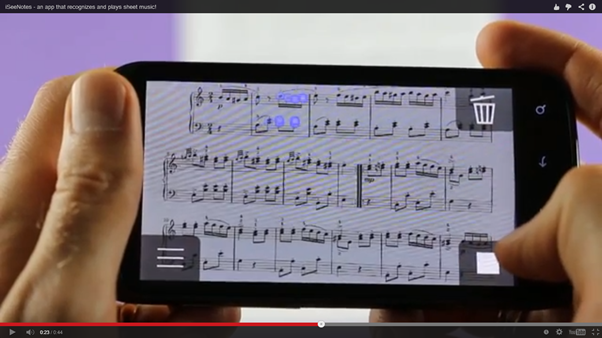
\includegraphics[width=120mm]{./assets/iseenotes.png}
    \caption{iSeeNotes Demo}
    \label{iseenotes}
\end{figure}

\begin{figure}[ht!]
    \centering
    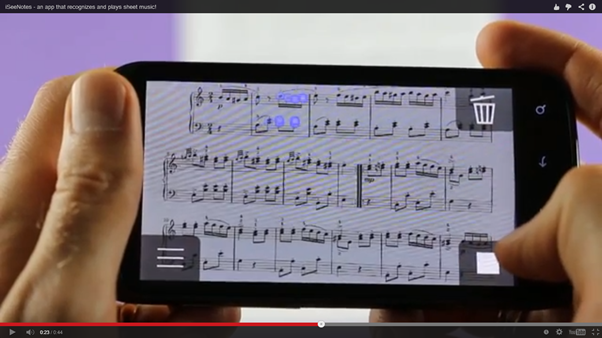
\includegraphics[width=120mm]{./assets/iseenotes.png}
    \caption{iSeeNotes Demo}
    \label{iseenotes}
\end{figure}

\begin{itemize}
  \item A singer is learning to sight read music. He can take a picture of the sheet music with the app and it will play the notes so they can learn them.
  \item A saxophonist wants to play a duet but finds herself alone, she takes a picture of the accompaniment with the app and it plays the piano part.
  \item A child learning to read music, uses the app to bring the sheet music to life
  \item A Trumpet player needs to transpose a piece in to Bb from concert key, and our app allows them to capture the music, and then shift the pitch in any number of existing applications, without having to laboriously manually input each note into a music notation program.
  \item A musician has a printed copy of some music, but wants to archive it or share it. Our app could allow them to do this, and actually enhance the original quality of the sheet music.
\end{itemize}

There are existing OMR solutions on the marketplace, however they primarily deal with scanned or computer generated images and run on desktop computers. There are very few mobile OMR applications.

One of the select few is �iSeeNotes�, an Android application by �Gear Up AB�  that was actually mentioned in our project brief. We ran this application on a simple piece of sheet music, �Baa Baa Black Sheep�, and found that, whilst it processed quickly, the results were quite unreliable. In our trials, roughly 80% of notes were accurately detected. Despite computer vision being a notoriously difficult problem we felt there is significant room for improvement.

INSERT ISEENOTES PICTURE with caption: "A snapshot from the iSeeNotes promotional video"

\subsection{Objectives}
The main difference between desktop OMR products and mobile ones, is that photograph from a mobile device imaging is significantly lower quality than a scanned image. Consider the following issues.

\begin{itemize}
  \item Lighting tolerant: Our application should be able to scan images even where uniform lighting isn�t possible
  \item Distortion tolerant: Our application should be able to correct unavoidable perspective distortion found in even the highest quality photos.
  \item Resolution: Most flatbed scanners support resolutions of at least 1200ppi, meaning a typical A4 scan could contain 140 megapixels. In comparison most mobile phones have an order of magnitude less megapixels.
\end{itemize}

In addition to these issues, mobile devices have much less processing power than desktop PCs but our users need to be able to expect sheet music in a reasonable amount of time. Our target maximum processing time was decided at 10 seconds, though this changed over the course of the project. 

Therefore our primary objective was to make an OMR application that can adapt to the constraints imposed by a mobile environment.

\subsection{Achievements}
We have created application that can reliably detect and interpret the foundations of music notation. In  particular, we have a robust solution for the recognition of staves and basic notes, even dealing with moderate levels of non-uniform perspective distortion. This also runs well within our 30 second time criteria, even processing complex sheet music on a 2011 device that would be considered slow by today�s standards.

Additionally, our app exports music to the MIDI format, which is the industry standard format for music sequences. Exporting in this format means that the users of our app can now continue to use the music information they�ve created in many other music applications.

We have also implemented detection of more advanced musical features to a reasonable degree of accuracy considering the difficulties involved in this task. This will be explained in greater detail throughout the report.

All of this can be done portably using an android device. We have also managed to keep the response times within reasonable bounds.
